
\begin{figure}[ht!]
    \centering
    
\resizebox{0.75\columnwidth}{!}{


\tikzset{every picture/.style={line width=0.75pt}} %set default line width to 0.75pt        

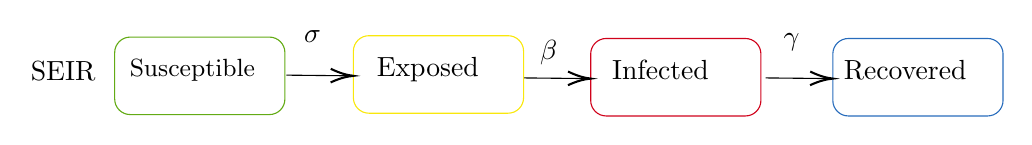
\begin{tikzpicture}[x=0.75pt,y=0.75pt,yscale=-1,xscale=1]
%uncomment if require: \path (0,300); %set diagram left start at 0, and has height of 300

%Rounded Rect [id:dp9217887491174969] 
\draw  [color={rgb, 255:red, 99; green, 171; blue, 21 }  ,draw opacity=1 ] (62.33,41.47) .. controls (62.33,37.34) and (65.68,34) .. (69.8,34) -- (136.87,34) .. controls (140.99,34) and (144.33,37.34) .. (144.33,41.47) -- (144.33,63.87) .. controls (144.33,67.99) and (140.99,71.33) .. (136.87,71.33) -- (69.8,71.33) .. controls (65.68,71.33) and (62.33,67.99) .. (62.33,63.87) -- cycle ;
%Rounded Rect [id:dp36097559929859013] 
\draw  [color={rgb, 255:red, 208; green, 2; blue, 27 }  ,draw opacity=1 ] (291.67,42.13) .. controls (291.67,38.01) and (295.01,34.67) .. (299.13,34.67) -- (366.2,34.67) .. controls (370.32,34.67) and (373.67,38.01) .. (373.67,42.13) -- (373.67,64.53) .. controls (373.67,68.66) and (370.32,72) .. (366.2,72) -- (299.13,72) .. controls (295.01,72) and (291.67,68.66) .. (291.67,64.53) -- cycle ;
%Straight Lines [id:da9742211892376831] 
\draw    (259.33,53.67) -- (289.67,53.98) ;
\draw [shift={(291.67,54)}, rotate = 180.59] [color={rgb, 255:red, 0; green, 0; blue, 0 }  ][line width=0.75]    (10.93,-3.29) .. controls (6.95,-1.4) and (3.31,-0.3) .. (0,0) .. controls (3.31,0.3) and (6.95,1.4) .. (10.93,3.29)   ;
%Rounded Rect [id:dp37752716490425275] 
\draw  [color={rgb, 255:red, 40; green, 108; blue, 188 }  ,draw opacity=1 ] (408.33,42.13) .. controls (408.33,38.01) and (411.68,34.67) .. (415.8,34.67) -- (482.87,34.67) .. controls (486.99,34.67) and (490.33,38.01) .. (490.33,42.13) -- (490.33,64.53) .. controls (490.33,68.66) and (486.99,72) .. (482.87,72) -- (415.8,72) .. controls (411.68,72) and (408.33,68.66) .. (408.33,64.53) -- cycle ;
%Straight Lines [id:da2512507786148114] 
\draw    (376,53.67) -- (406.33,53.98) ;
\draw [shift={(408.33,54)}, rotate = 180.59] [color={rgb, 255:red, 0; green, 0; blue, 0 }  ][line width=0.75]    (10.93,-3.29) .. controls (6.95,-1.4) and (3.31,-0.3) .. (0,0) .. controls (3.31,0.3) and (6.95,1.4) .. (10.93,3.29)   ;
%Rounded Rect [id:dp4832950812851634] 
\draw  [color={rgb, 255:red, 249; green, 231; blue, 9 }  ,draw opacity=0.99 ] (177.33,40.8) .. controls (177.33,36.68) and (180.68,33.33) .. (184.8,33.33) -- (251.87,33.33) .. controls (255.99,33.33) and (259.33,36.68) .. (259.33,40.8) -- (259.33,63.2) .. controls (259.33,67.32) and (255.99,70.67) .. (251.87,70.67) -- (184.8,70.67) .. controls (180.68,70.67) and (177.33,67.32) .. (177.33,63.2) -- cycle ;
%Straight Lines [id:da02397316252168946] 
\draw    (145,52.33) -- (175.33,52.65) ;
\draw [shift={(177.33,52.67)}, rotate = 180.59] [color={rgb, 255:red, 0; green, 0; blue, 0 }  ][line width=0.75]    (10.93,-3.29) .. controls (6.95,-1.4) and (3.31,-0.3) .. (0,0) .. controls (3.31,0.3) and (6.95,1.4) .. (10.93,3.29)   ;


% Text Node
\draw (68.33,43.33) node [anchor=north west][inner sep=0.75pt]   [align=left] {{\small Susceptible}};
% Text Node
\draw (300.67,44) node [anchor=north west][inner sep=0.75pt]   [align=left] {Infected};
% Text Node
\draw (412.33,44) node [anchor=north west][inner sep=0.75pt]   [align=left] {Recovered};
% Text Node
\draw (266,34.07) node [anchor=north west][inner sep=0.75pt]    {$\beta $};
% Text Node
\draw (383.33,31.07) node [anchor=north west][inner sep=0.75pt]    {$\gamma $};
% Text Node
\draw (187.33,42.67) node [anchor=north west][inner sep=0.75pt]   [align=left] {Exposed};
% Text Node
\draw (152.33,29.73) node [anchor=north west][inner sep=0.75pt]    {$\sigma $};
% Text Node
\draw (20.67,44.33) node [anchor=north west][inner sep=0.75pt]   [align=left] {SEIR};


\end{tikzpicture}

}
    \caption{Diagram of a dynamic compartmental model.}
    \label{fig:dynamicmodel} 
\end{figure}